%------------
%------------
\chapter{PCA}

% apriori Algorithmus nicht sinnvoll, aber evtl erste Überlegung, da er Implikationen findet, die evtl gewollter Eingabe ähneln

 \todo{einheitliche Benennung von PCA Dimension, erhobenen Daten etc.}

 Eine \emph{Principal Component Analysis} (PCA) oder auch Hauptkomponentenanalyse wir auf einer Menge von Datenpunkten (oder Beispielen) mit jeweils $n$ Dimensionen ausgeführt. Sie findet diejenigen Richtungen im $n$-dimensionalen Raum, in denen sich die Beispiele am meisten unterscheiden, die "`principal components"'. Das Ziel ist in den meisten Fällen die Dimensionalität der Daten zu reduzieren. Das wird dadurch erreicht, dass die Eingabedaten nur noch durch die "`principal components"' dargestellt werden, da die anderen Dimensionen optimalerweise nur einen marginalen Einfluss auf die Daten haben.
 
 Das Ziel im Bezug auf die Generierung von Skeletten war vor allem die Position und Krümmung der Wirbelsäule bei unterschiedlichen Tieren zu untersuchen, da diese sehr charakteristische Merkmale eines Skeletts sind. Aus dem gleichen Grund soll der Algorithmus zur Generierung der Skelette mit der Generierung der Wirbelsäule starten und daraus dann den Rest der Knochen "`wachsen"' lassen.
 Die Hoffnung hier ist auch, dass dadurch Skelette generiert werden, die ausbalanciert wirken. Es soll nichts generiert werden, das aussieht, als würde es sofort umfallen. \todo{Hat das funktioniert?}
 
 Eine PCA, die als Eingabe viele Beispiele für Wirbelsäulen und ein paar weiteren Daten zum zugehörigen Tier bekommt, ist hier hilfreich, da sie Zusammenhänge für die Positionierung der Wirbelsäule liefert.
 
 
 %-----------------------
 \section{Funktionsweise}
 
 \todo{PCA Quelle} % Folien? Oder besser Standardwerk zitieren?
 \todo{PCA-Algorithmus mit Pseudocode und Ein- und Ausgabe als Referenz (Eingabe ist Kovarianzmatrix, Rest Vorberechnung?)}
 
 Die Eingabe für eine PCA ist eine Menge von Punkten. Diese Punkte repräsentieren einzelne Instanzen dessen, was untersucht werden soll. Hier sind die Datenpunkte Skelette von Wirbeltieren. Für jede Eigenschaft des Skeletts, die untersucht werden soll, hat der Punkt eine Dimension. Gegeben ist also eine Menge von Punkten mit jeweils $n$ Dimensionen. Die PCA nimmt an, dass die Punkte in jeder Dimension normal-/gaußverteilt sind. In diesem Fall bilden die Punkte im $n$-dimensionalen Raum einen Ellipsoid.
 
 Das Ziel der PCA ist herauszufinden wo die Achsen des Ellipsoids liegen, also wie die Eingabedimensionen miteinander korreliert sind. Interessant sind dabei die Achsen in deren Richtung die Daten die größe Streuung aufweisen.
 
 Um diese Achsen zu berechnen, wird zunächst die Kovarianzmatrix aufgestellt, deren Einträge die Kovarianz zwischen den verschiedenen Achsen beschreibt.
 Die Eigenvektoren dieser Kovarianzmatrix sind dann die Achsen des Ellipsoids und die zugehörigen Eigenwerte geben an wie groß die Varianz in dieser Richtung ist, also wie weit ausgedehnt das Ellipsoid in dieser Richtung ist. Der Mittelpunkt des Ellipsoids ist der Mittelwert der Daten.
 
 Will man nun herausfinden was die Haupteigenschaften eines Datenpunktes sind, stellt man ihn im neuen Koordinatensystem des Ellipsoids dar, also als gewichtete Summe der Eigenvektoren. Dann betrachtet die Dimensionen mit den größten Eigenwerten. Dazu zieht man zunächst den Mittelwert vom Datenpunkt ab und multipliziert ihn dann mit der transponierten Basiswechselmatrix, also der Matrix, in der in den Zeilen die Eigenvektoren stehen.


 %---------------------- 
 \section{Datenerhebung}
 
 Die konkret erhobenen Beispiele sind vor allem der Datenlage \bzw der zugänglichen Quellen geschuldet. Trotzdem wurde darauf geachtet möglichst viele unterschiedliche Tierarten mit viel Variation in den erhobenen Merkmalen zu finden.
 
 Viele Beispiele stammen Zoologiebüchern, in denen sie als Beispiele für bestimmte Erklärungen angegeben waren (Bildquellen siehe Anhang \ref{appendix_pca_skeletons}). Dem ist auch geschuldet, dass recht viele Dinosaurierskelette dabei sind. Denn von anderen Tieren gibt es als alternative Darstellungsmöglichkeit eine Außenansicht des lebenden Tieres. Das geht bei ausgestorbenen Tieren im Allgemeinen nicht.
 
 Die Merkmale, die zur Datenerhebung ausgesucht wurden, sind charakteristisch für ein Skelett, tragen also viel zum Gesamteindruck bei. Das sind vor allem der Verlauf der Wirbelsäule und der Aufbau der Extremitäten.
  
 Eingeschränkt wurde die Erhebung natürlich auch durch die begrenzte Datenlage. Am einfachsten zu bekommen sind 2D-Bilder mit Seitenansichten von Skeletten. Das schließt Merkmale aus, die Tiefeninformationen benötigen, \zb den Abstand der Füße oder die Winkel der Gelenke an den Beinen. Auch Informationen zu sehr kleinen Knochen, wie Handwurzelknochen oder die unterschiedlichen Fingerknochen, sind schwierig zu bekommen, da sie teilweise schwierig zu Erkennen und zu Markieren sind. Deshalb haben wir die Erhebung auf folgende Daten eingeschränkt:
  
 \begin{itemize}
  \item Ein Bild mit der Seitenansicht des Skeletts.
  Darin wurde die Lage der Wirbelsäule und die Länge der Knochen der Vorder- und Hintergliedmaßen markiert, falls vorhanden.
  
  \item Die Tierklasse, also ob das Tier ein Fisch, ein Amphib, ein Reptil oder ein Säugetier ist. Dieses Merkmal lässt sich nicht auf einer kontinuierlichen Skala abbilden und ist deshalb nicht als Eingabedimension für die PCA geeignet. Es wurde trotzdem erhoben, da es für eine anderweitige Auswertung hilfreich sein könnte.
  
  \item Ob Flügel vorhanden sind ("`ja"' repräsentiert durch die Zahl eins und "`nein"' repräsentiert durch null).
  
  \item Die Anzahl der Beine mit Bodenkontakt.
  
  \item Das ungefähre Gewicht eines ausgewachsenen Exemplars des Tieres, zu dem das Skelett gehört, in Kilogramm. Hier wurde oft das maximale Gewicht verwendet, da keine Angaben zum Durchschnittsgewicht zu finden waren. Teilweise gibt es auch verschiedene (Unter-)Arten, die unterschiedlich schwer werden können, deren Skelette aber, bei der Auflösung der hier erhobenen Daten, gleich aussehen. In diesem Fall wurde ein beliebiger Wert gewählt, der zwischen dem Gewicht der leichtesten und dem der schwersten (Unter-)Art liegt. (Die Quellen zu den Gewichten sind im Anhang \ref{appendix_pca_weight} zu finden.)
 \end{itemize}

 Die Bilder der Skelette wurden folgendermaßen für die Datenerhebung vorbereitet:
 
 \begin{enumerate}
  \item Zuschneiden des Bildes, so dass möglichst nur das Skelett mit wenig Rand außen herum zu sehen ist.
  \item Einfügen in eine $1000 \times 1000$ Pixel große Bildumgebung.
  \item Verschieben innerhalb der Bildumgebung an den unteren Rand und horizontal in die Mitte.
 \end{enumerate}

 Ist das geschehen kann die Lage der Wirbelsäule und die Länge der Knochen der Extremitäten annotiert werden. Details dazu wie die Daten annotiert und ausgelesen wurden sind in Abschnitt \ref{section_pca} zu finden.
 
 Die Lage der Wirbelsäule wird durch drei kubische Bézierkurven erfasst. Jeweils einer für Hals, Rücken und Schwanz. Hals und Rücken gehen an der Schulter ineinander über und Rücken und Schwanz beim Becken.
 Diese Bézierkurven sind die ersten $20$ Eingabedimensionen für die PCA ($10$ zweidimensionale Punkte). Bei manchen Tieren ist kein Hals oder kein Schwanz vorhanden. In diesen Fällen werden die $3$ fehlenden Punkte jeweils mit dem ersten \bzw letzten Punkt des Rückens ersetzt.
 
 Zusätzlich wird jeweils durch eine Gerade im Bild die Länge des Ober- und Unterarms, der Hand, des Ober- und Unterschenkels und des Fußes eingetragen, falls vorhanden. Die Bezeichnung der Extremität als Arm oder Bein ist nur zur Unterschiedung zwischen Vorder- und Hinterextremitäten gedacht. Sie hat in keiner Weise etwas mit der Funktion der Gliedmaßen zu tun.
 
 Zusätzlich zum Bild gibt es noch eine Textdatei, in der die anderen Daten, die oben schon erwähnt wurden, erfasst werden.
 
 Bei der Annotation der Bilder sind folgende Schwierigkeiten aufgetreten:
 \todo{in Text einbetten}
 
 \begin{itemize}
  \item Bei Fischen ist nicht klar wo Rücken in Schwanz übergeht, da der Beckengürtel sich teilweise beim Kopf befindet oder auch gar nicht vorhanden ist. Bei der Datenerhebung wurde der Übergang ungefähr bei der Rücken- oder der Afterflosse festgelegt, da dies relativ gut zum Algorithmus passt.
  
  \item Hals und Schwanz von manchen Tieren ist mit einer kubischen Bézierkurve nicht darstellbar. Das ist unter den verwendeten Beispielen der Hals von Ichthyornis und vom Schwan und der Schwanz vom Ichthyosaurus und vom Koboldmaki. In diesem Fällen wurde versucht die Form möglichst gut anzunähern oder Fortsätze (wie am Schwanz vom Ichthyosaurus) die im Algorithmus wahrscheinlich sowieso nicht abgebildet werden, einfach wegzulassen.
  
  \item Die Schwanzposition bei Tieren mit sehr langen Schwänzen ist auf den Bildern relativ beliebig. Hier wurde versucht den Schwanz möglichst gerade nach hinten fortzusetzen, auch wenn er auf dem Bild irgendwie eingerollt ist.
 \end{itemize}
 
 %---------------------------------
 \section{Analyse der Eingabedaten}
 \label{pca_input_analysis}
 
  Insgesamt wurden $44$ Datenpunkte erhoben. Das entspricht bei $29$ Dimensionen $44 \cdot 44 = 1276$ Zahlen als Eingabe. Das Ergebnis der PCA ist im wesentlichen die $29 \times 29$ große Kovarianzmatrix. Das sind $841$ \bzw $\frac{29 \cdot 30}{2} = 435$ Zahlen als Ausgabe. Da $1276 < 435$, ist das eine ausreichende Menge an erhobenen Beispielen. \todo{bessere Begründung?}
 
 Der Mittelwert aller Eingabedaten ist in Abbildung \ref{mean} visualisiert.
 \todo{Werte der Mittelwertvisualisierung angeben wenn zuletzt aktualiert, damit Bild nicht so groß sein muss; und Rand abschneiden}
 Wie die bei der Datenerhebung ist hier die Position der Wirbelsäule auf einem $1000 \times 1000$ Pixel Bild gezeigt. Da von den Knochen der Beine und Arme nur die Längen erhoben wurden, sind ihre Positionen nicht realistisch. Die Ober- und Unterschenkel und die Ober- und Unterarme, sind von den Übergangspunkten Hals-Rücken und Rücken-Schwanz senkrecht nach unten gezeichnet, Hand und Fuß sind vom jeweiligen Endpunkt von Arm oder Bein horizontal nach links gezeichnet. Die restlichen Daten sind nicht visualisiert, sondern nur in Textform in der oberen linken Ecke angegeben.
 
 Eine Vorraussetzung dafür, dass die PCA korrekt funktionert, ist, dass die Eingabedaten in jeder Dimension normalverteilt sind. Im Folgenden sollen die Eingabemerkmale daraufhin genauer untersucht werden.
 
 Es gibt die beiden Merkmale \emph{Flügel} und \emph{Beine mit Bodenkontakt}, die offensichtlich nicht normalverteilt sind, da sie diskret nur ein \bzw zwei Werte annehmen können. Sie können jedoch hilfreiche Informationen zur Weiterverarbeitung durch den Algorithmus liefern, weshalb sie nicht ganz außen vor gelassen werden sollten. Da das Hauptaugenmerk der PCA aber auf der Position der Wirbelsäule und dem Aufbau der Extremitäten liegen soll, sollen diese beiden Merkmale keinen großen Einfluss haben. Deshalb wurden diese Merkmale kleinskaliert. Dazu weiter unten mehr.
 
 Die anderen Dimensionen wurden mithilfe eines Quantil-Quantil-Diagramms mit der Normalverteilung verglichen. 
 \todo{QQ Diagramme erklären, negative Werte sind ganz normal, da inverse CDF bei einem Mittelwert von 0 bei Werten < 0.5 negativ ist.}
 Die Diagramm zeigen für alle Merkmale außer dem Gewicht, dass sie mehr oder weniger gut normalverteilt sind (siehe Beispiele in Abbildung \ref{qqdiagram_examples} und eine vollständige Aufzählung im Anhang in den Abbildungen \ref{qq_diagrams_spine} und \ref{qq_diagrams_rest}).
 
 Das Merkmal \emph{Gewicht} ist überhaupt nicht normalverteilt (siehe Abbildung \ref{qqdiagrams_weight} a und b). Verwendet man es als Eingabe für die PCA und generiert dann zufällig normalverteilte Punkte im Ergebnisraum, treten schnell Gewichte kleiner null auf.
 
 Betrachtet man das Gewicht jedoch auf einer logarithmischen Skala, so ist es wieder normalverteilt (siehe Abbildung \ref{qqdiagrams_weight} c). Deshalb wird das Gewicht zunächst logarithmiert, bevor es in die PCA eingeht.
 Welcher Logarithmus hier zur Umrechnung der Daten verwendet wird schlägt sich nur als linearer Faktor nieder und ist eine Frage der Skalierung. Es wurde der Zehnerlogarithmus verwendet. Eine solche Skalierung bestimmt die "`Wichtigkeit"' des Merkmals für die PCA. Da das Gewicht, wie die Merkmale \emph{Flügel} und \emph{Beine mit Bodenkontakt} nicht die Hauptmerkmale sind, die hier untersucht werden sollen, wurde es ebenfalls kleinskaliert.
 
 \begin{figure}
  \subfloat[x-Wert der $3$. Koordinate des Halses]{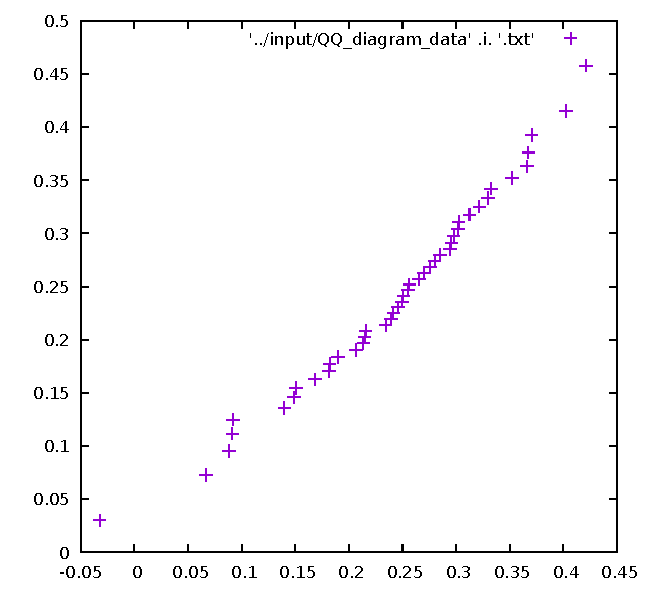
\includegraphics[width=0.3\textwidth]{../PCA/gnuplot/results_qq_diagrams/QQ_diagram4.pdf}}
  \qquad
  \subfloat[Länge der Hand]{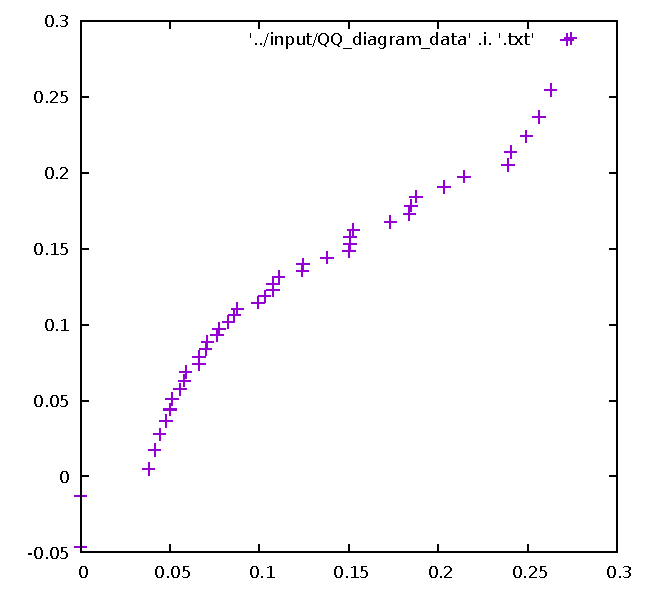
\includegraphics[width=0.3\textwidth]{../PCA/gnuplot/results_qq_diagrams/QQ_diagram24.pdf}}
  \qquad
  \subfloat[Länge des Oberschenkels]{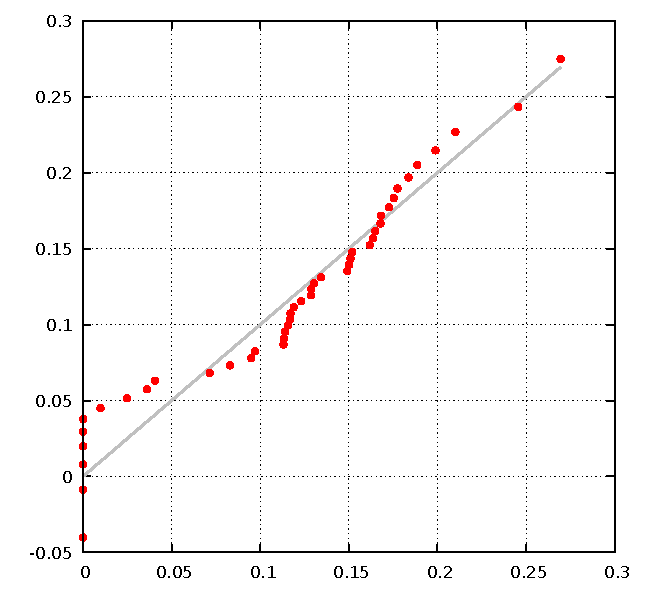
\includegraphics[width=0.3\textwidth]{../PCA/gnuplot/results_qq_diagrams/QQ_diagram25.pdf}}
  
  \caption{Beispielhaft ausgewählte Quantil-Quantil-Diagramme von drei Eingabedimensionen. (a) weicht nicht stark von der Normalverteilung ab, (b) und (c) hingegen schon mehr, sind aber trotzdem noch akzeptabel verteilt.}
  \label{qqdiagram_examples}
 \end{figure}
 
\begin{figure}
  \subfloat[Gewicht linear]{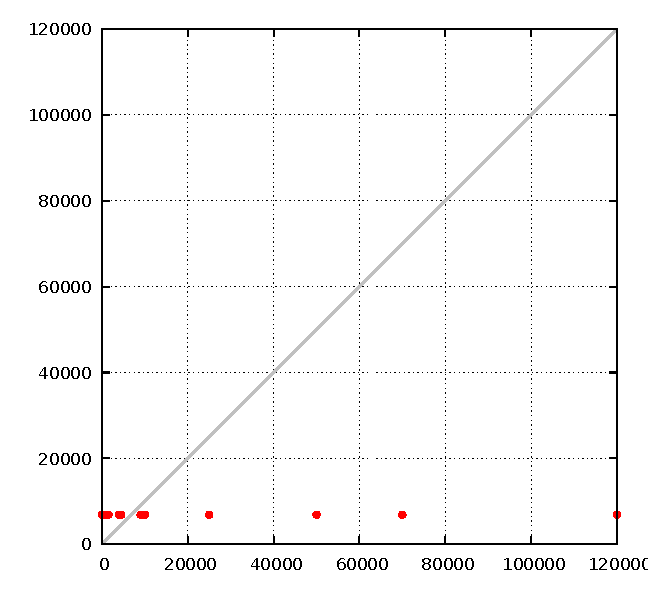
\includegraphics[width=0.3\textwidth]{../PCA/gnuplot/results_qq_diagrams/QQ_diagram_linear_weight.pdf}}
  \qquad
  \subfloat[Gewicht linear (Ausschnitt)]{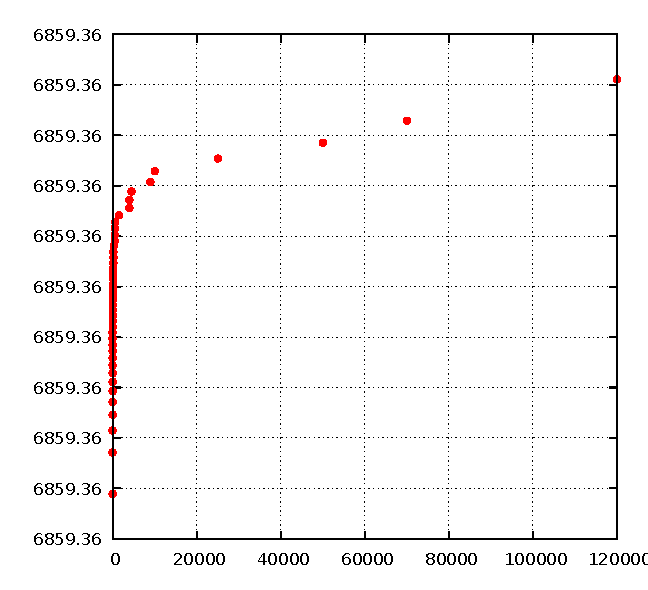
\includegraphics[width=0.3\textwidth]{../PCA/gnuplot/results_qq_diagrams/QQ_diagram_linear_weight_without_diagonal.pdf}}
  \qquad
  \subfloat[Gewicht logarithmisch]{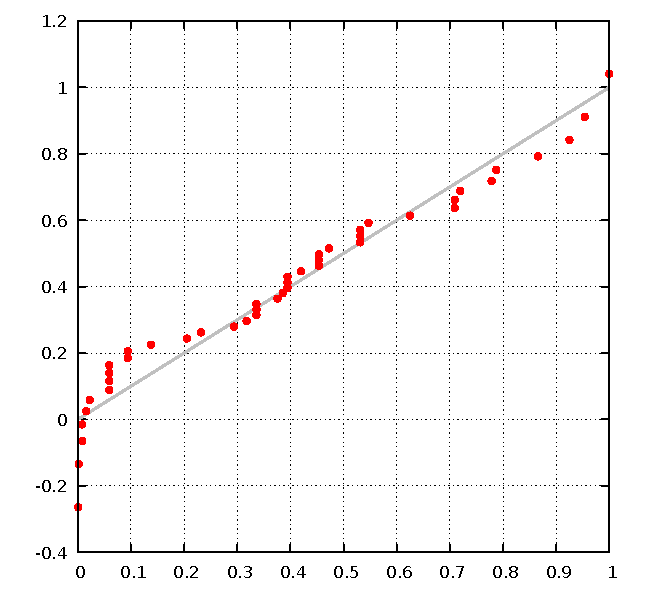
\includegraphics[width=0.3\textwidth]{../PCA/gnuplot/results_qq_diagrams/QQ_diagram28.pdf}}
  
  \caption{ Quantil-Quantil-Diagramme des Gewichts, einmal linear (a,b) und einmal mit logarithmischer Skala (b)}
  \label{qqdiagrams_weight}
 \end{figure}
 
 Generell bewirkt die Skalierung einer Dimension eine Gewichtung. Denn durch eine Skalierung ändert sich auch die (Co-)Varianz und somit auch die Kovarianzmatrix. Seien beispielsweise $s,t \in \mathbb{R}$, dann bewirkt eine Skalierung mit $s$ in Dimension $x$ und eine Skalierung mit $t$ in Dimension $y$ eine Skalierung von $s \cdot t$ der Kovarianz Cov$(x,y)$ von $x$ mit $y$, da $\mathrm{Cov}(sx, ty) = (sx - s\mu_x) (ty - t\mu_y) = st \cdot \mathrm{Cov}(x,y)$, mit Erwartungswert $\mu_i$ in Dimension $i$.
 
 Wie genau wurden nun die einzelnen Merkmale nur skaliert?
 
 Zunächst wurden alle Merkmale auf das Intervall $[0, 1]$ skaliert, damit alle den gleichen Einfluss haben.
 Bei Koordinaten oder Längen im Bild bedeutet das, dass sie mit $1000$ skaliert werden, da sie alle im Intervall $[0, 1000]$ liegen, da sie in Pixeln dargestellt werden und das Bild eine Größe von $1000 \times 1000$ Pixel hat. Bei Längen wären theoretisch auch Werte $> 1000$ möglich. Solche Längen wären aber unrealistisch und werden deshalb ignoriert.
 Koordinaten und Längen im Bild sind diejenigen Merkmale, die uns am meisten interessieren. Deshalb sollten sie den größten Einfluss auf das Ergebnis der PCA haben. Alle anderen Merkmale wurden deshalb kleiner skaliert.
 
 Man könnte statt einer Skalierung durch $1000$ auch für jedes einzelne Merkmal den maximal und minimal angenommenen Wert ermitteln und sie dann so skalieren, dass sie Intervalle gleicher länge abdecken. Das würde ausgleichen, dass \zb kleine Längen eine kleinere Varianz und damit auch einen kleineren Einfluss haben.
 Wir haben uns aber für die oben beschriebene Variante entschieden, da es natürlich wirkt, dass kleine Merkmale im Bild auch weniger wichtig sind. Falls in Zukunft Gründe für eine andere Gewichtung auftauchen ließe sich das aber leicht anpassen.
 
 Die diskreten Merkmale \emph{Flügel} und \emph{Beine mit Bodenkontakt} und das logarithmische Gewicht wurden zunächst ebenfalls auf das Intervall $[0, 1]$ skaliert. Das bedeutet für das Gewicht $w$: $\frac{\mathrm{log}(w+1)}{\mathrm{log}(\mathrm{max}+1)}$. Das schwerste Wirbeltier ist der Blauwal mit bis zu 120 Tonnen (siehe \ref{appendix_pca_weight}). Deshalb ist hier max $= 120.000$.
 
 Danach wurden die Werte noch einmal durch $100$ geteilt, um ihren Einfluss zu verringern. Das Ziel war, dass diese Merkmale nicht als große Einträge in den ersten paar Eigenvektoren auftauchen. Ohne diese Skalierung sind diese Merkmale recht dominant. Mit der Skalierung hingegen sind sie in den größten Eigenvektoren unter den kleinsten Werten zu finden.
 
 Berachtet man nun die so skalierten Eingabedaten, so hat der Klippschliefer den minimalen Abstand zum Mittelwert (siehe Abbildung \ref{klippschliefer_farbig}). Zusätzlich zum Bild wurde für den Klippschliefer folgende Daten erhoben:
 \emph{Tierklasse} Säugetier, \emph{Flügel} nein, \emph{Anzahl Beine mit Bodenkontakt} $4$, \emph{Gewicht} $4$kg.
 
 Den maximalen Abstand hat die Schlange. Die erhobenen Daten sind hier:
 \emph{Tierklasse} Reptil, \emph{Flügel} nein, \emph{Anzahl Beine mit Bodenkontakt} $0$, \emph{Gewicht} $50$kg. Die Schlange ist allerdings das einzige Tier zu dem es kein Bild des Skeletts gibt. Das liegt daran, dass es keine seitlichen Abbildungen von ausgestreckten Schlangen gibt. Sie werden eigentlich immer gekrümmt dargestellt, da sonst das Bild sehr lang und schmal werden würde. Deshalb wurde für die Schlange nur eine horizontale Gerade knapp über dem unteren Bildrand eingezeichnet, die den Rücken darstellen soll. Extremitäten und ersichtliche Punkte an denen der Rücken in Hals oder Schwanz übergeht gibt es ja keine.
 
 Der Punkt mit dem zweitgrößten Abstand zum Mittelwert ist das Känguru (siehe Abbildung \ref{kaenguru_farbig}). Zusätzlich zum Bild gibt es hier folgende Daten:
  \emph{Tierklasse} Säugetier, \emph{Flügel} nein, \emph{Anzahl Beine mit Bodenkontakt} $2$, \emph{Gewicht} $50$kg
 
  \begin{figure}
  \centering
  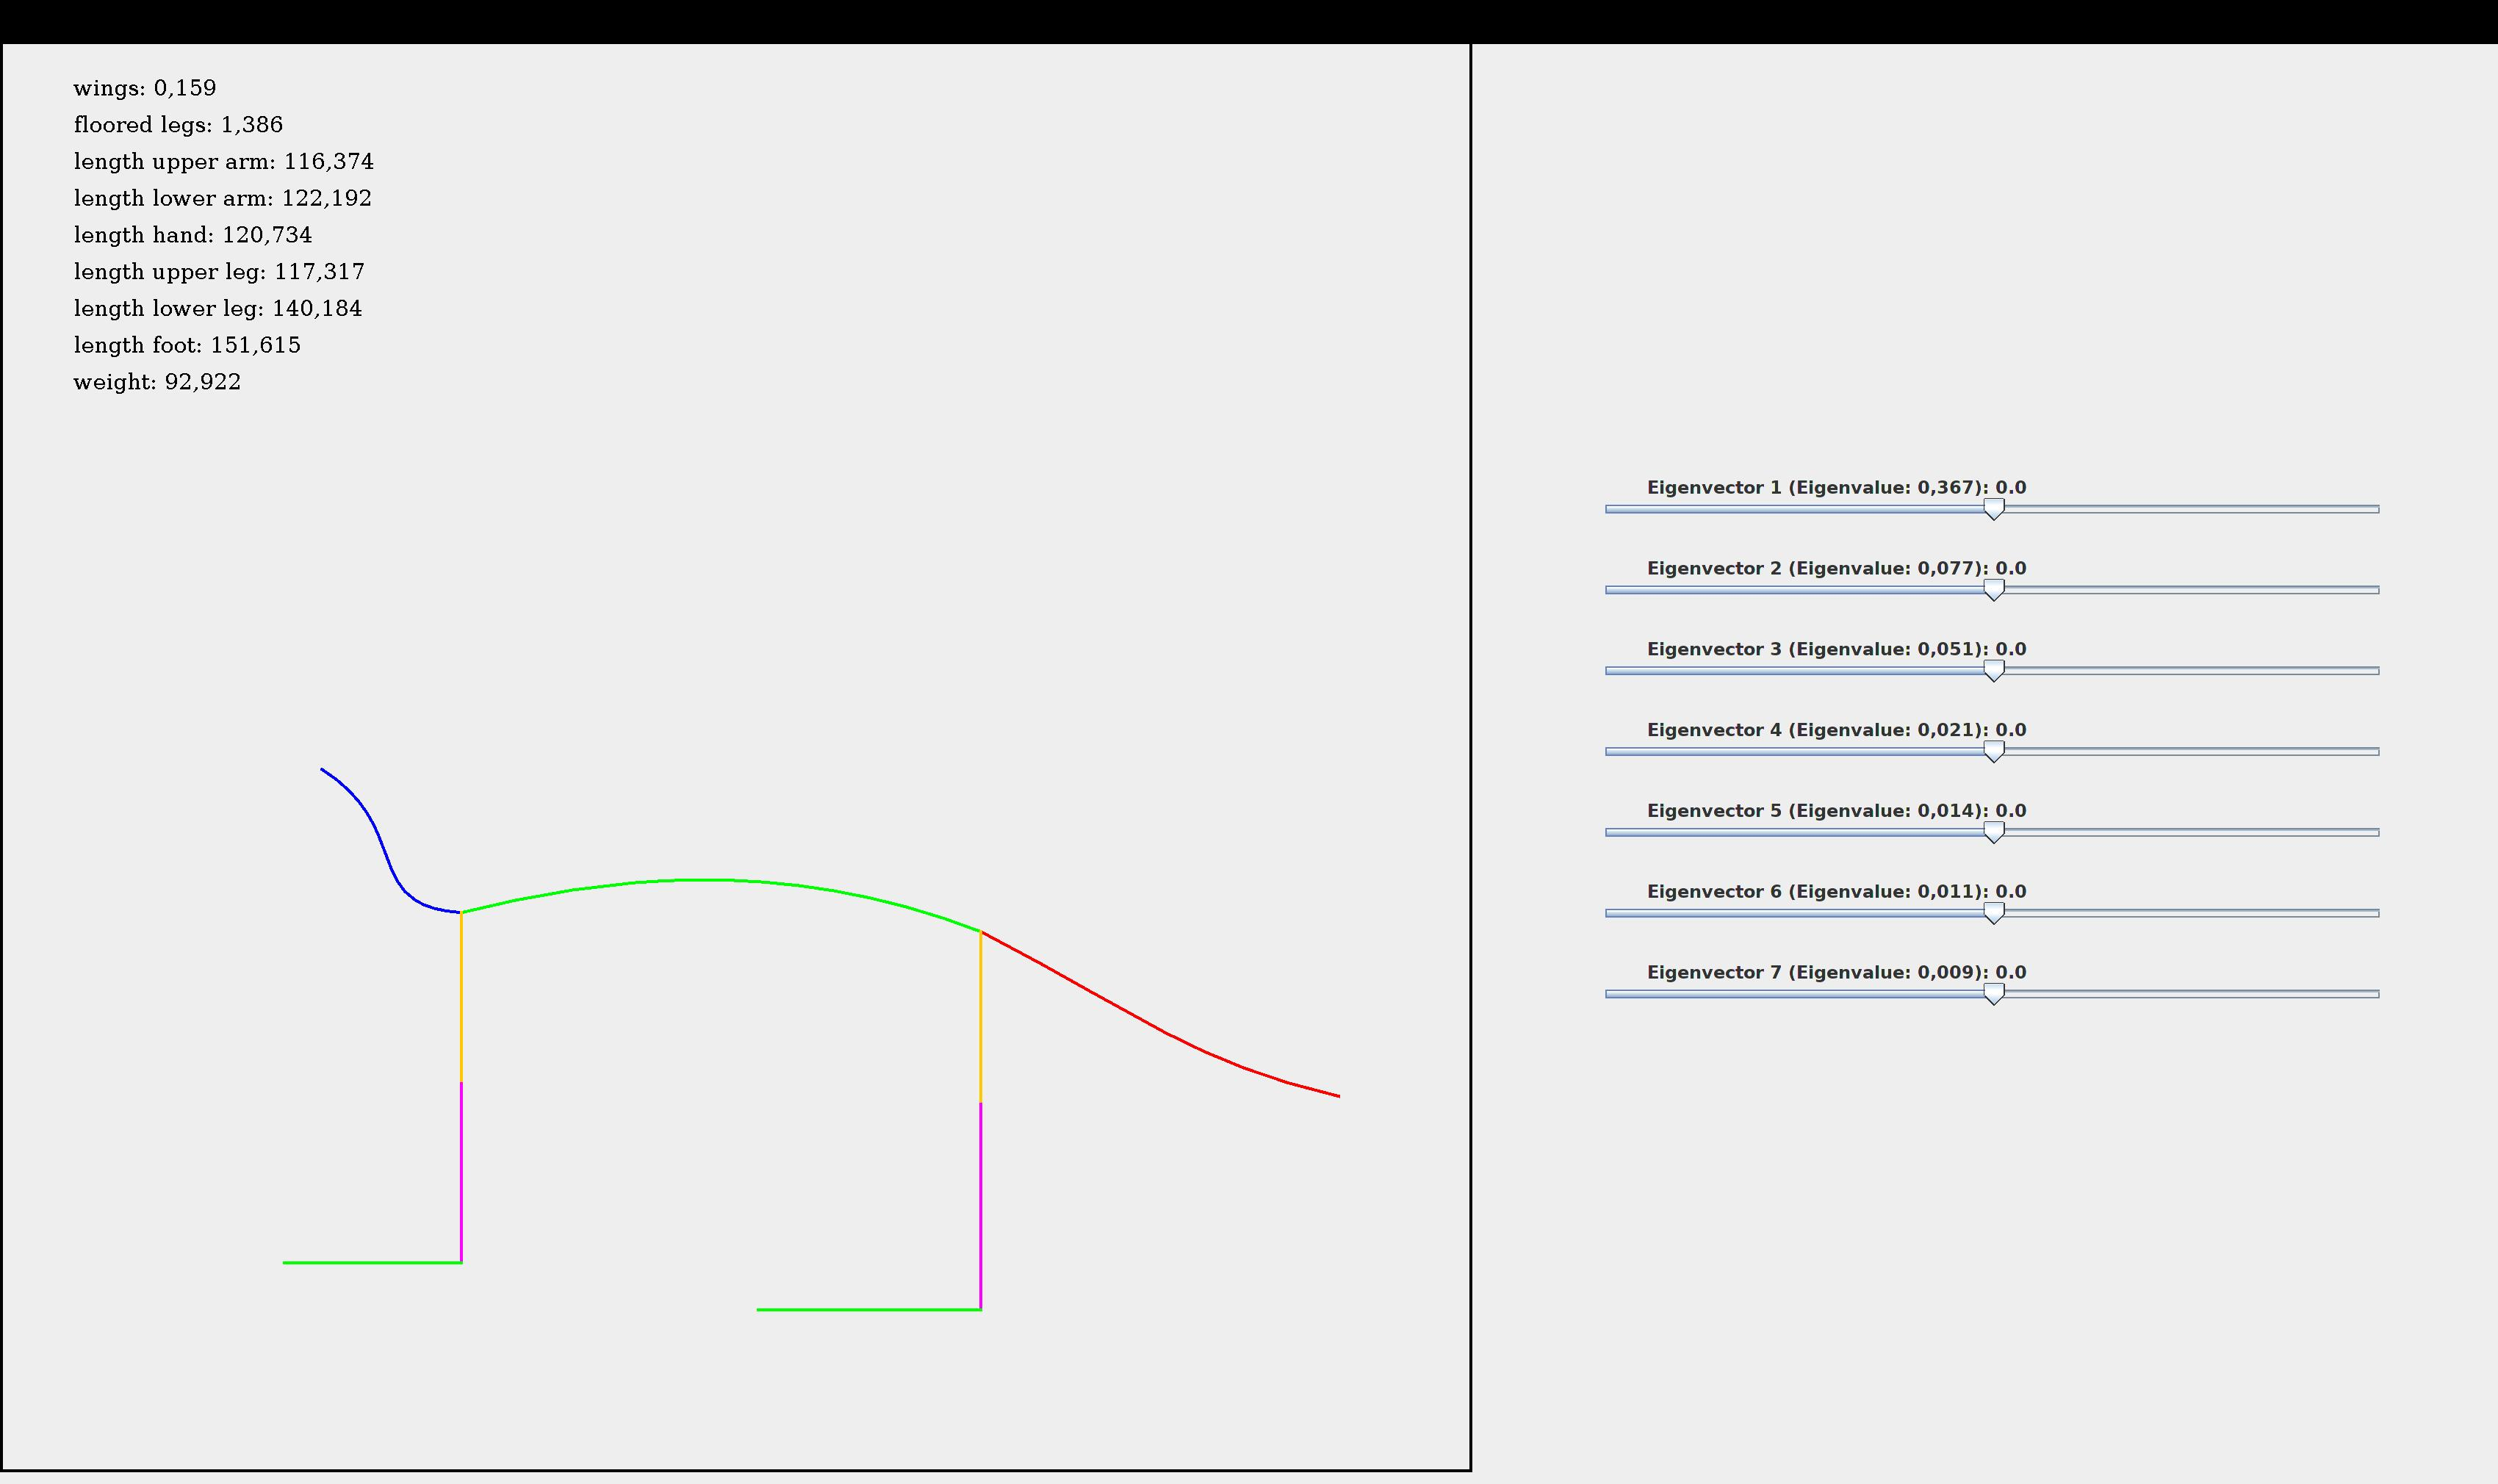
\includegraphics[width=0.9\textwidth]{../PCA/mean_log_weight_downscaled_wings_legs_and_weight.jpg}
  \caption{Visualisierung des Mittelwerts der Eingabedaten. Die Werte, die nicht visualisiert sind, sind folgende: ...}
  \label{mean}
 \end{figure}
 
 \begin{figure}
  \subfloat[Klippschliefer]{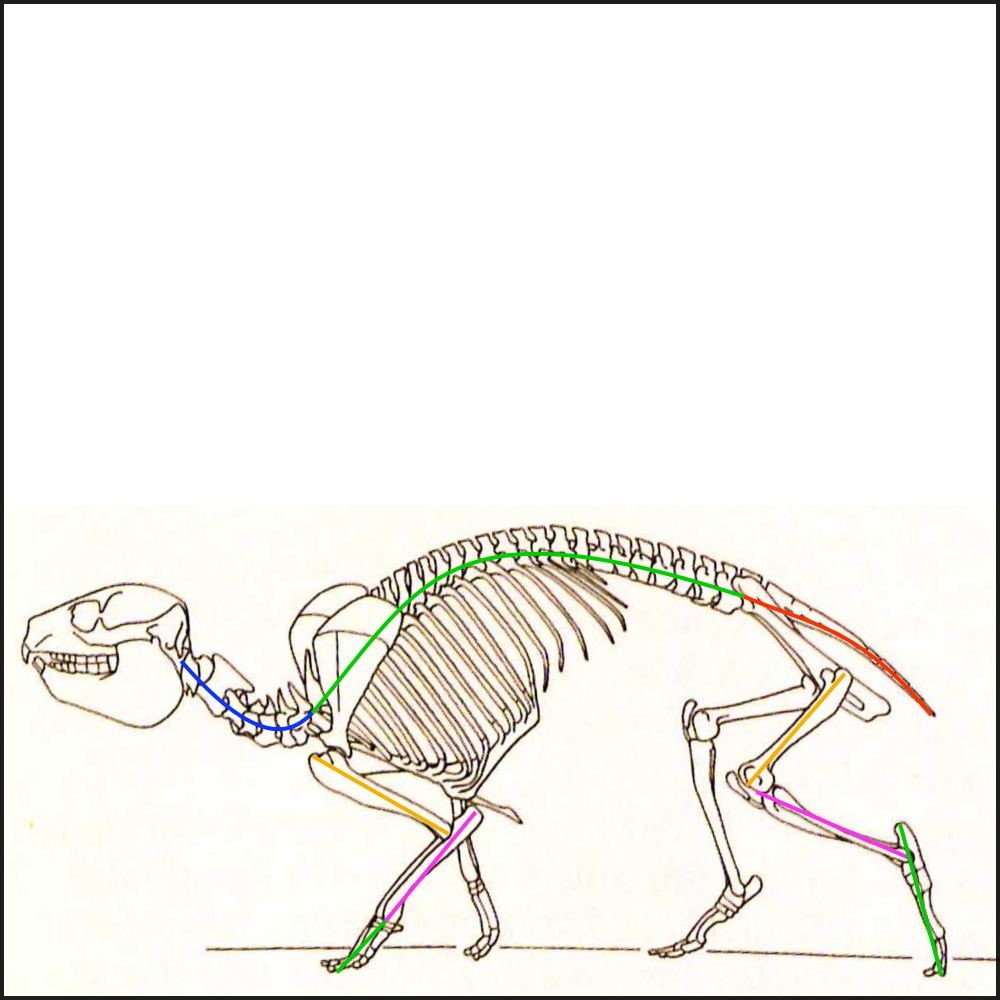
\includegraphics[width=0.5\textwidth]{../PCA/Skelettbilder/Klippschliefer_farbig.png} \label{klippschliefer_farbig}}
  \qquad
  \subfloat[Känguru]{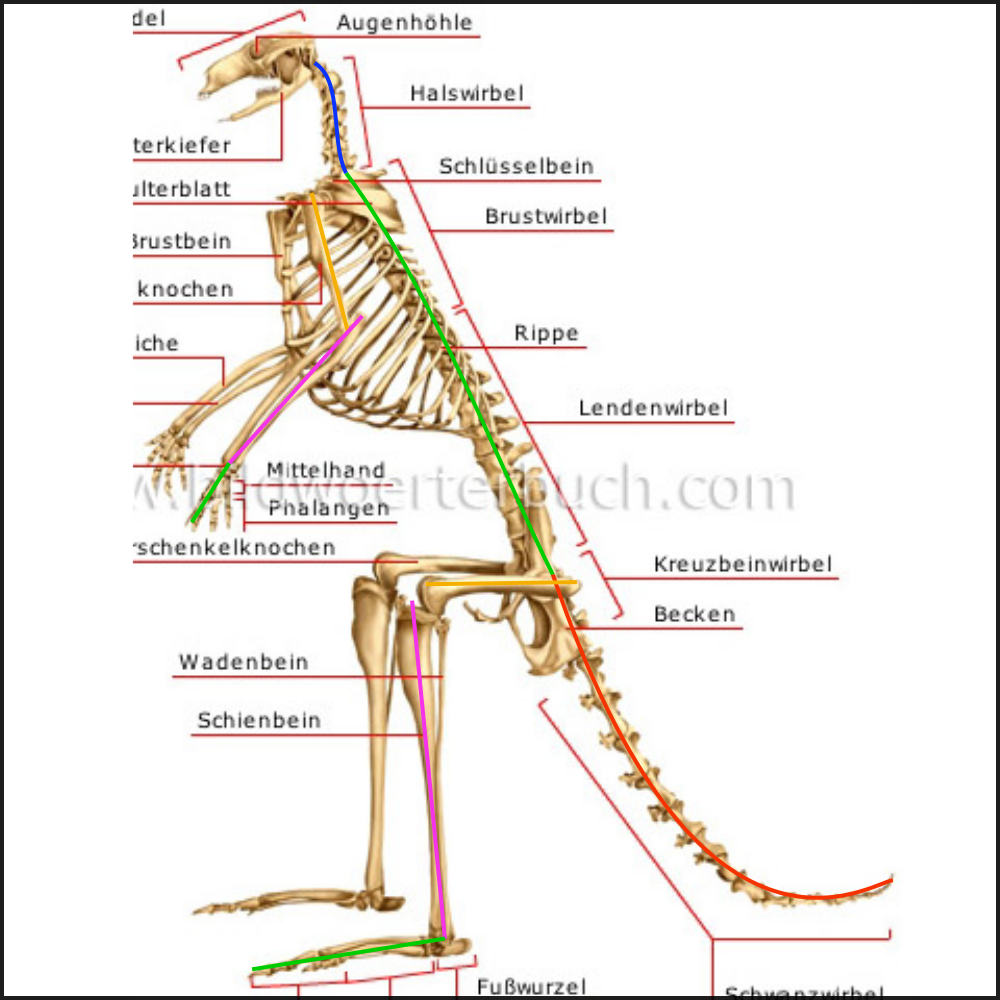
\includegraphics[width=0.5\textwidth]{../PCA/Skelettbilder/Kaenguru_farbig.png}\label{kaenguru_farbig}}
  
  \caption{Annotierte Bild des Skeletts eines Klippschliefers (a) und eines Kängurus(b). Die Teile der Wirbelsäule und die Knochen der Extremitäten sind hier jeweils mit der gleichen Farbe markiert wie in der Visualisierung des Mittelwerts (Abbildung \ref{mean})}
 \end{figure}

 
 Zuletzt betrachten wir noch die Projektion der Eingabedaten auf die ersten zwei  Eigenvektoren. In Abbildung \ref{projections_scales} ist noch einmal gut zu vergleichen was die Effekte der Skalierung der Eingabedaten ist. Ganz links sind die Ergenisse zusehen, die entstehen, wenn man alle Merkmale nur auf das Intervall $[0, 1]$ skaliert. In der Mitte geht das Gewicht nicht mehr linear, sondern logarithmisch ein und ganz rechts sind \emph{Flügel}, \emph{Anzahl Beine} und \emph{Gewicht} zusätzlich kleinskaliert. Gut zu sehen ist, wie sich die Clusterbildung durch die Anpassungen verringert.
 \todo{aAnpassung der Stile der Plots}
 
 In Abbildung \ref{projections_tags} ist nocheinmal jeweils die Projektion der Daten auf die ersten beiden Eigenvektoren zu sehen. Diesmal mit unterschiedlich markiert mit den diskret erhobenen Daten. Hier sieht man \zb schön dass alle Tiere mit Flügeln auch Vögel sind und dass fast alle Tiere mit zwei Beinen Vögel sind. Die vier Tiere, die zwei Beine haben, aber keine Vögel sind, sind die Ohrenrobbe, der Seehund, der Tyrannosaurus Rex und das Känguru.

 \begin{figure}
  \subfloat[gleiche Skalierung aller Dimensionen]{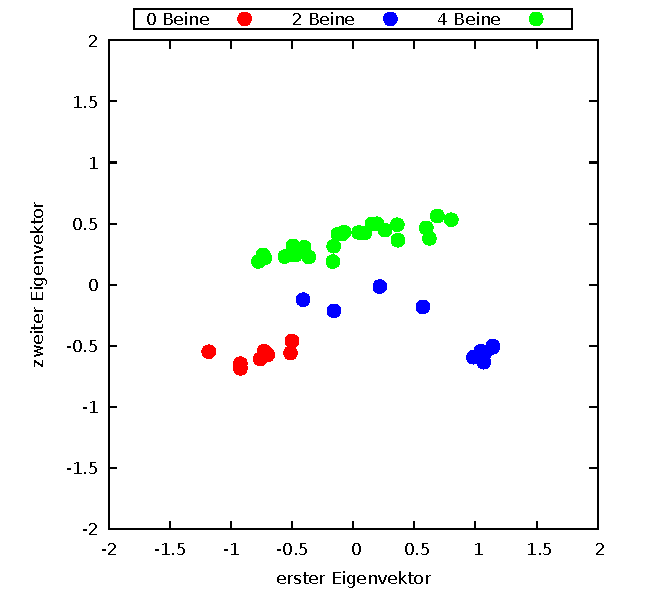
\includegraphics[width=0.3\textwidth]{../PCA/gnuplot/results_with_leg_tag/projection_eigenvectors12.pdf}}
  \qquad
  \subfloat[logarithmisches Gewicht]{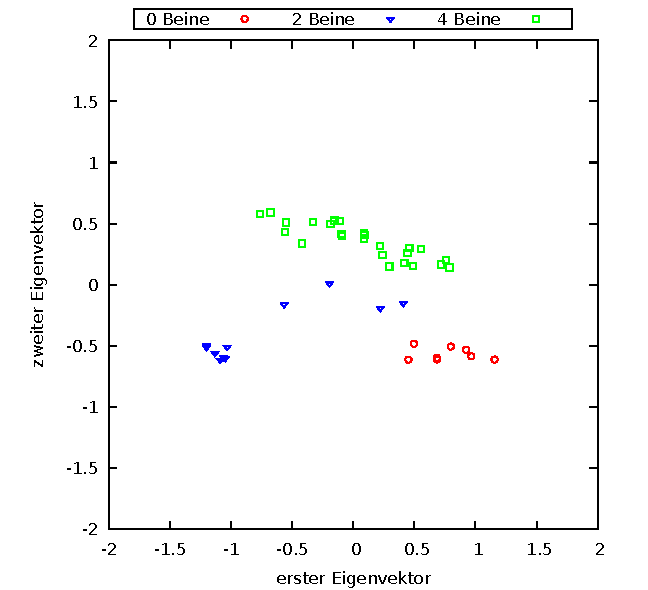
\includegraphics[width=0.3\textwidth]{../PCA/gnuplot_log_weight/results_with_leg_tag/projection_eigenvectors12.pdf}}
  \qquad
  \subfloat[skalierte "`Zusatzmerkmale"']{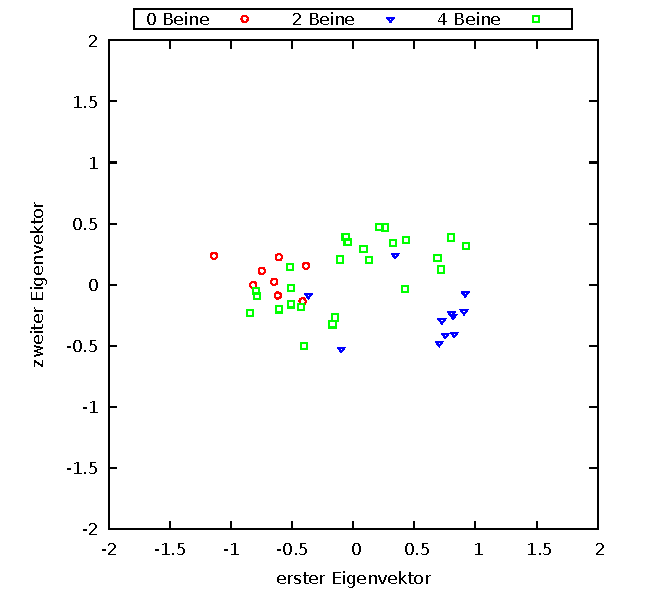
\includegraphics[width=0.3\textwidth]{../PCA/gnuplot_log_weight_with_downscaled_wings_legs_and_weight/results_with_leg_tag/projection_eigenvectors12.pdf}}
  
  \caption{Dargestellt sind hier jeweils die Projektionen der Eingabedaten auf die ersten beiden Eigenvektoren. Für jede Version wurden die Eingabedaten unterschiedlich vorverarbeitet. (a) Skalierung aller erhobenen Daten auf das Intervall $[0, 1]$, (b) zusätzlich Verwendung von logarithmischem Gewicht, statt linearem, (c) zusätzliche Skalierung der Merkmale \emph{Flügel}, \emph{Anzahl Beine} und \emph{Gewicht} durch $100$. In Version (b) wurde der erste Eigenvektor durch die PCA umgedreht, weshalb das Cluster der Zweibeiner auf der linken, statt der rechten Seite zu sehen ist.}
  \label{projections_scales}
 \end{figure}
 
 \begin{figure}
  \subfloat[Flügel]{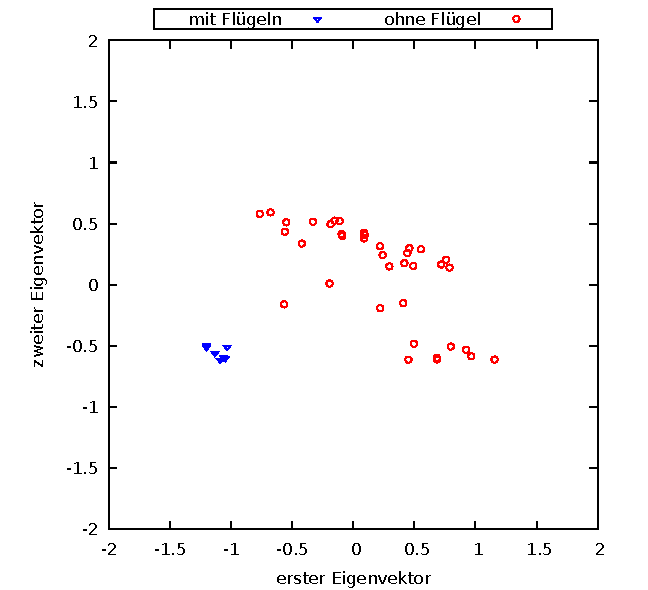
\includegraphics[width=0.3\textwidth]{../PCA/gnuplot_log_weight/results_with_wing_tag/projection_eigenvectors12.pdf}}
  \qquad
  \subfloat[Anzahl Beine mit Bodenkontakt]{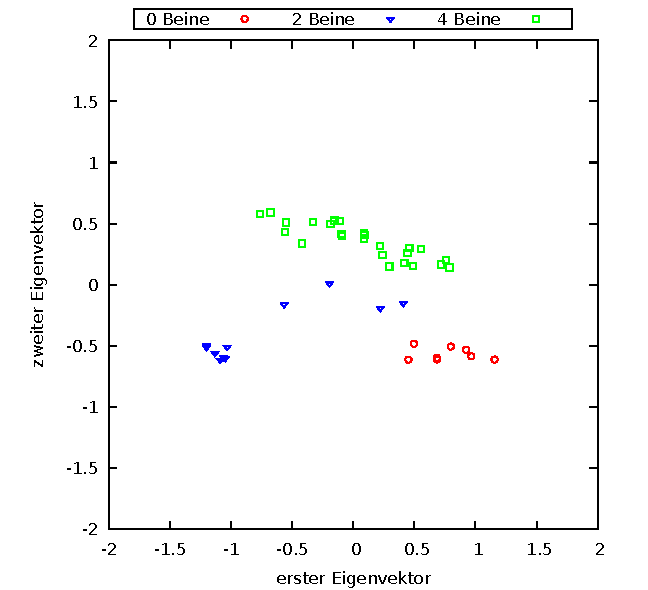
\includegraphics[width=0.3\textwidth]{../PCA/gnuplot_log_weight/results_with_leg_tag/projection_eigenvectors12.pdf}}
  \qquad
  \subfloat[Tierklasse]{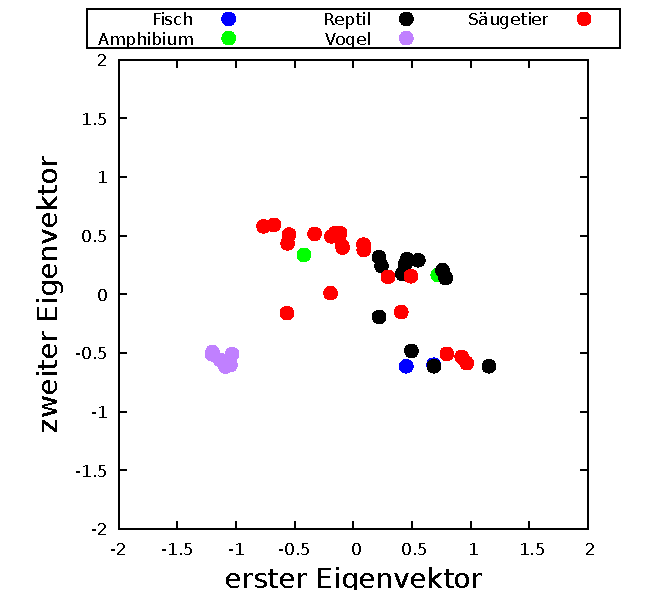
\includegraphics[width=0.3\textwidth]{../PCA/gnuplot_log_weight/results_with_animal_class_tag/projection_eigenvectors12.pdf}}
  
  \caption{Projektion der Eingabdaten auf die Ebene, die durch den ersten und zweiten Eigenvektor aufgespannt wird. Markiert sind jeweils verschiedene Merkmale der Punkte.}
  \label{projections_tags}
 \end{figure}
 

 %-----------------------------------
 \section{Analyse der PCA-Ergebnisse}
 \label{section_pca_result_analysis}
 
 Von $29$ Eingabedimensionen gibt es auch $29$ Eigenvektoren mit Eigenwerten größer $0$. Der kleinste hat einen Wert von $0,000024$. Von den Eigenwerten sind $7$ größer als $0,01$. Leider reichen diese $7$ Dimensionen aber noch nicht aus, um die Eingabedaten hinreichend anzunähern. Bei manchen Tieren funktioniert das ganz gut (siehe Archaeopteryx, Abbildung \ref{archaeopteryx}), bei anderen aber eher schlechter (siehe Frosch, Abbildung \ref{frosch}).
 \todo{updaten}
 Die Daten konnten somit von der PCA nicht besonders gut komprimiert werden. Trotzdem sind die berechneten Eigenvektoren hilfreich für die (Weiter-)Entwicklung des Algorithmus. \todo{wenn Algo weiterentwickelt, beschreiben}
 
 \begin{figure}
  \centering
  \subfloat[Rekonstruktion]{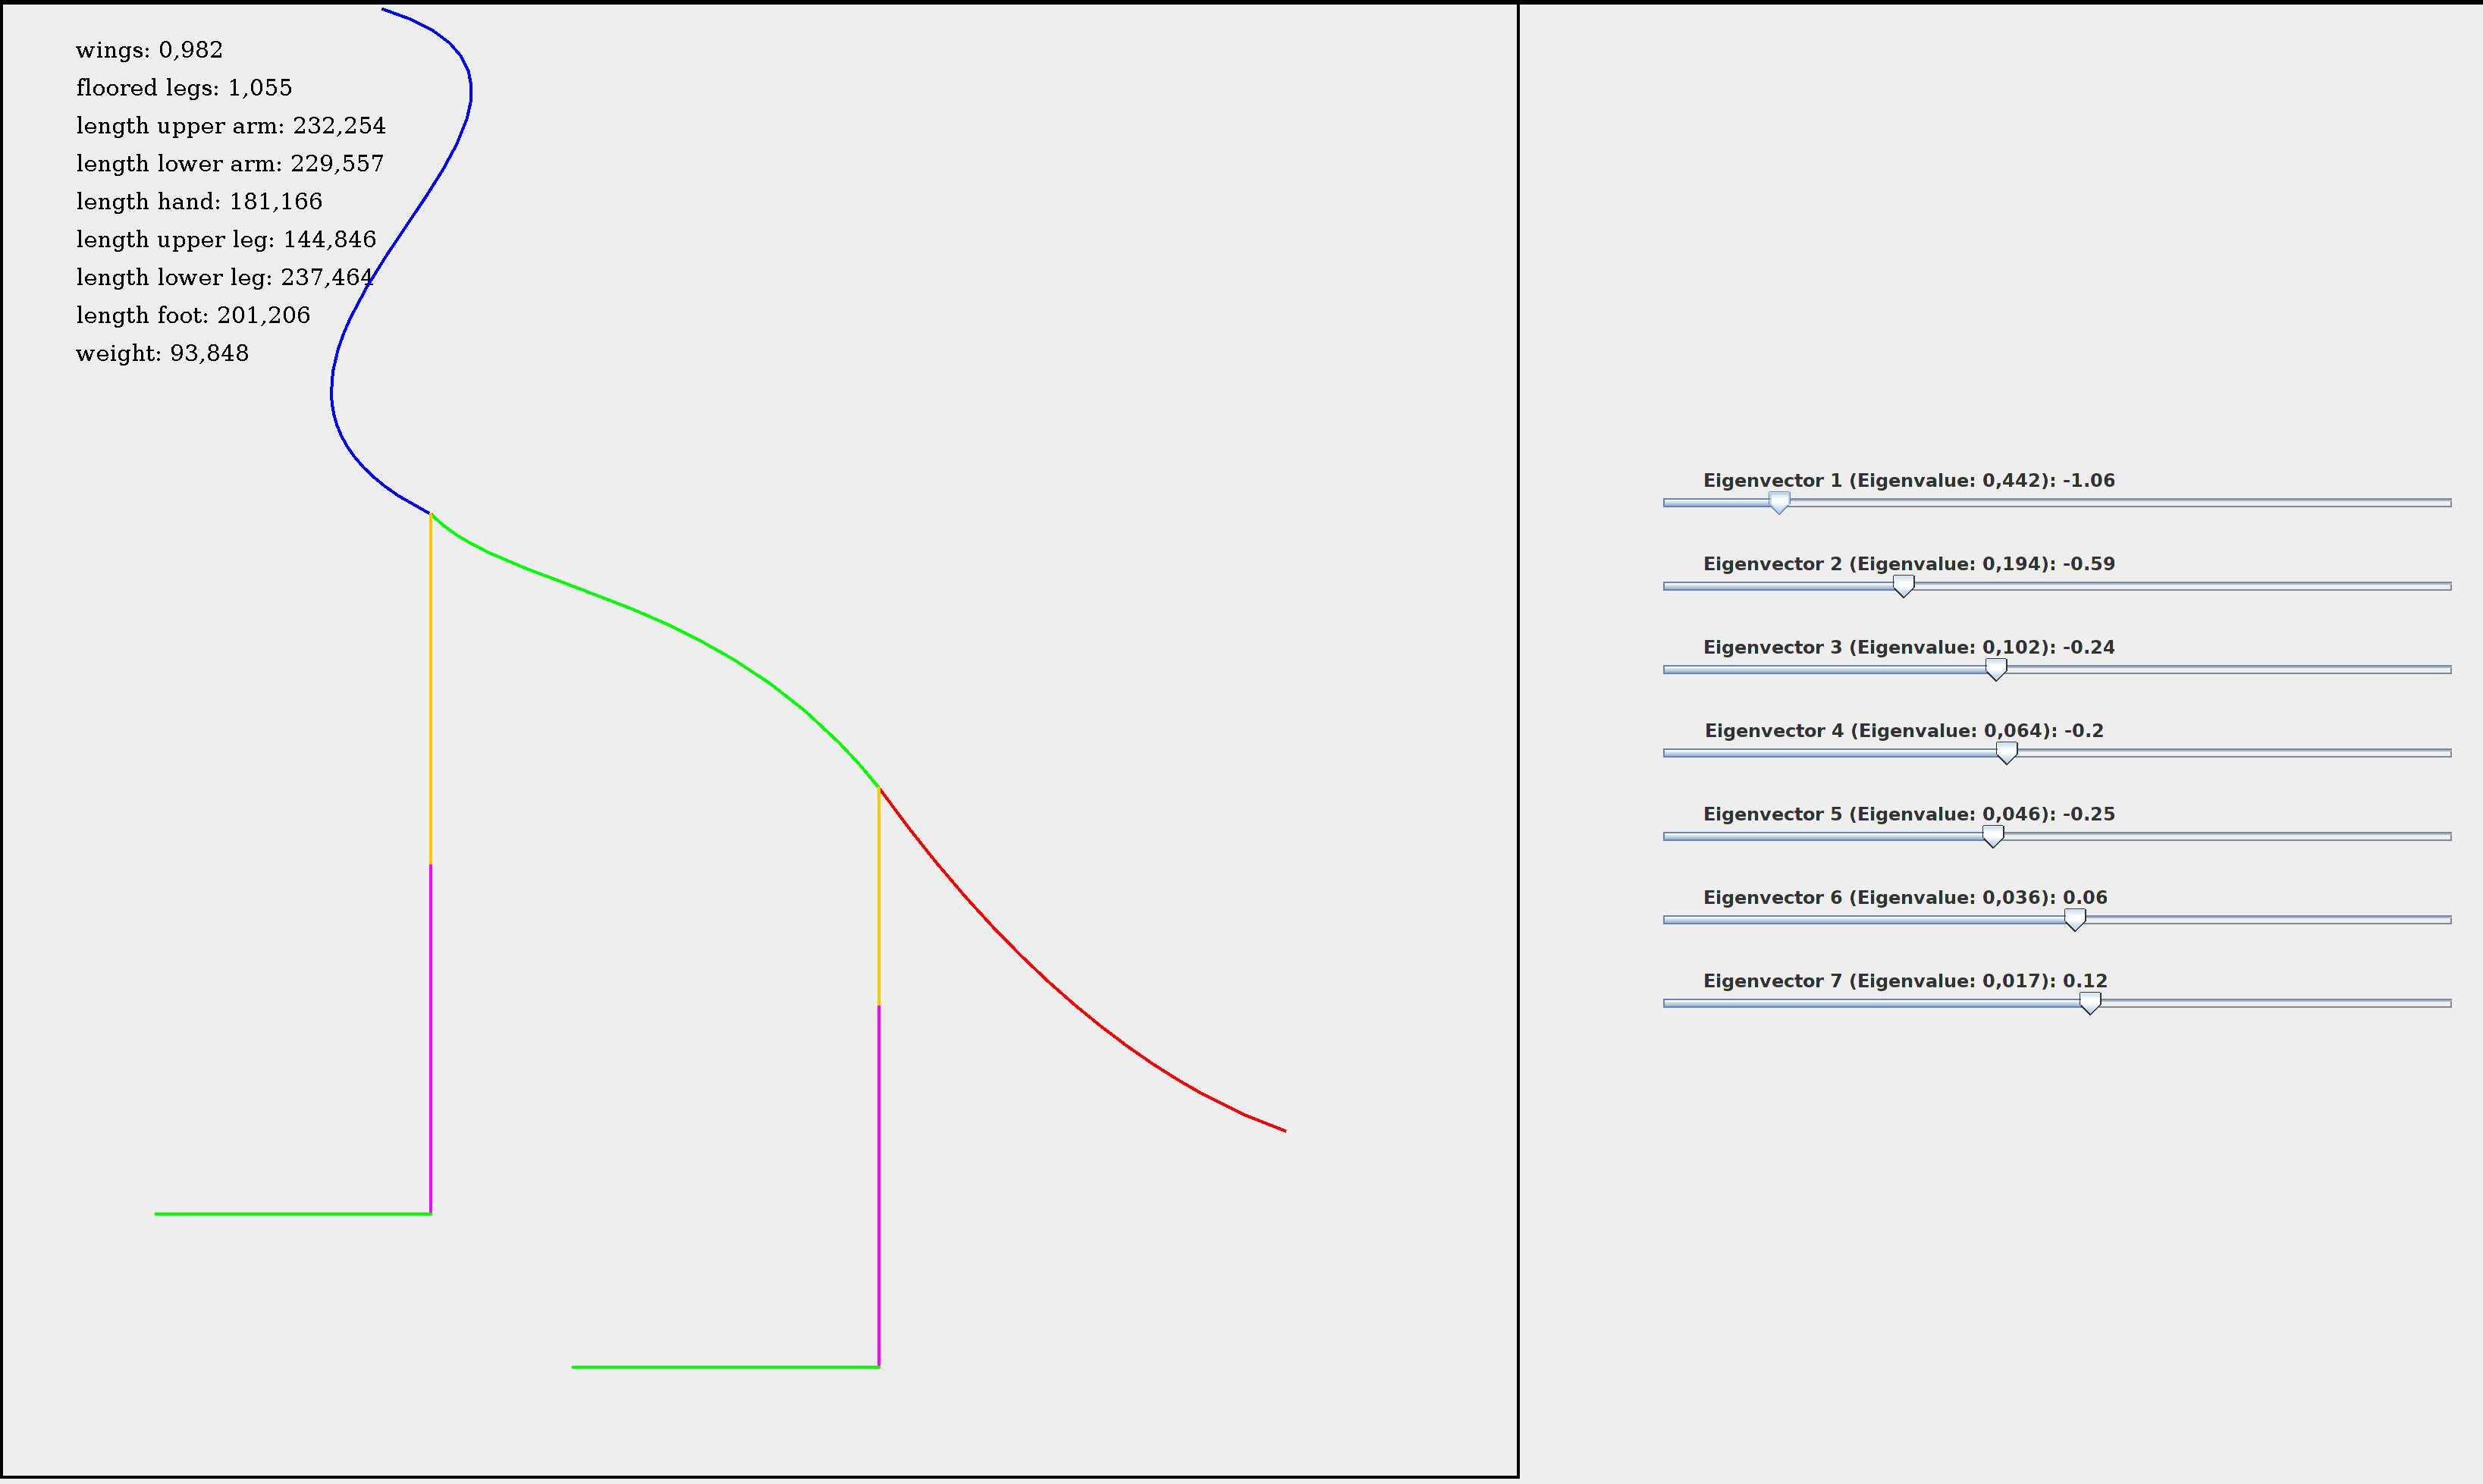
\includegraphics[width=\textwidth]{../PCA/animal_reconstructions_log_weight/Archaeopteryx.jpg}}
  \\
  \subfloat[Eingabebild]{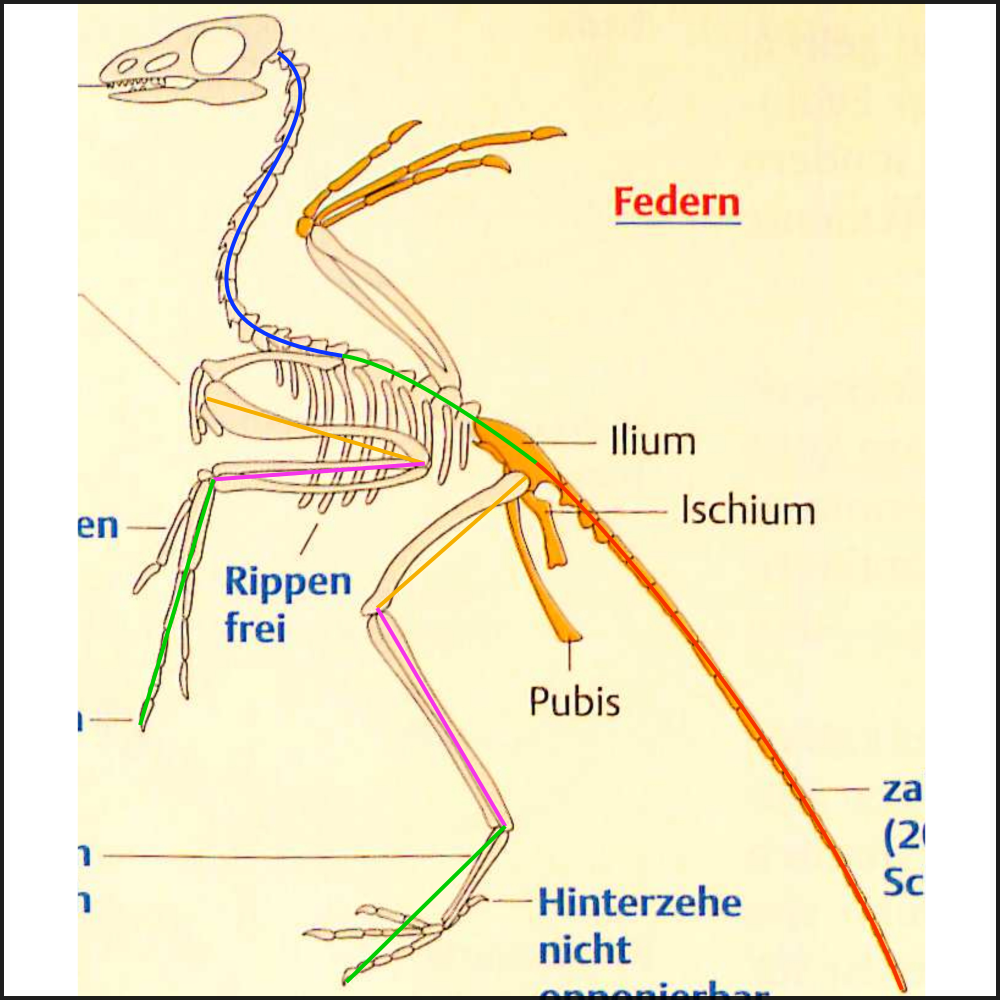
\includegraphics[width=0.5\textwidth]{../PCA/Skelettbilder/Archaeopteryx_farbig.png}}
  
  \caption{Archaeopteryx (a) Rekonstruktion aus den größten $7$ Eigenvektoren, (b) Eingabebild, zusätzlich erhobene Daten sind:
  Tierklasse: Vogel, Flügel, Paare von Beinen mit Bodenkontakt: $1$, ungefähres Gewicht: $1$kg}
  \label{archaeopteryx}
 \end{figure}
 
\begin{figure}
  \centering
  \subfloat[Rekonstruktion]{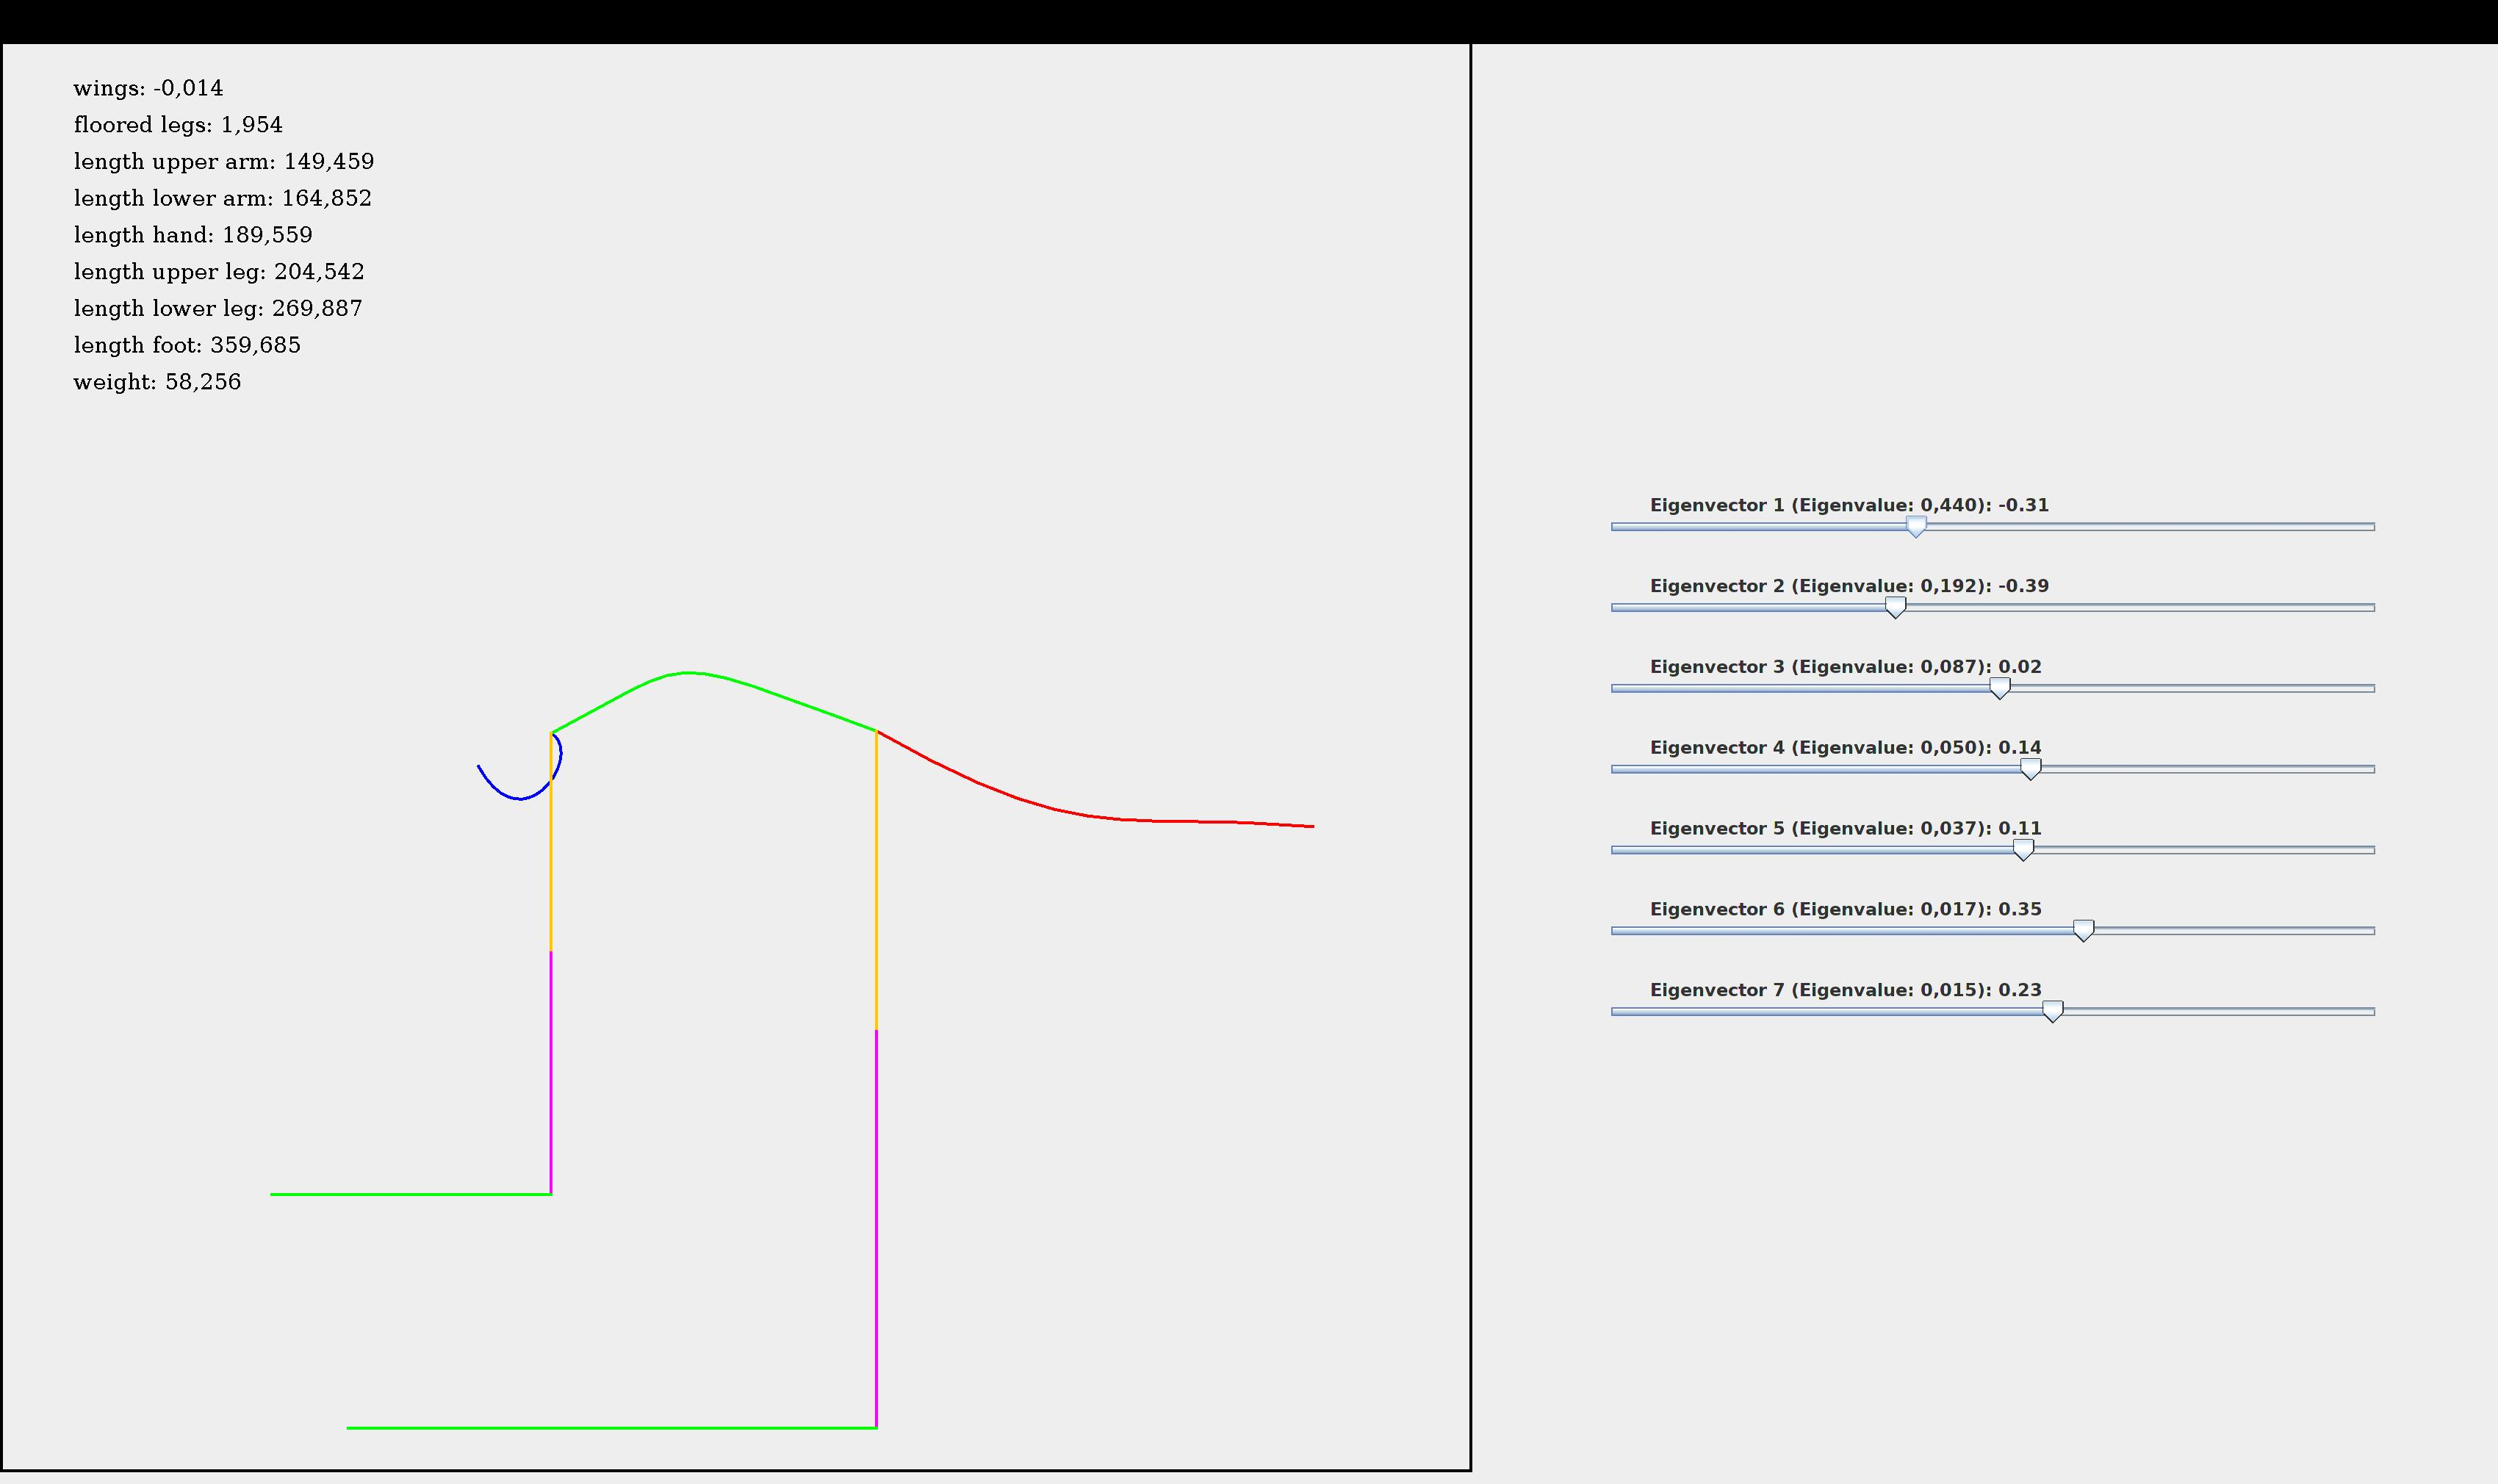
\includegraphics[width=\textwidth]{../PCA/animal_reconstructions_log_weight/Frosch.jpg}}
  \\
  \subfloat[Eingabebild]{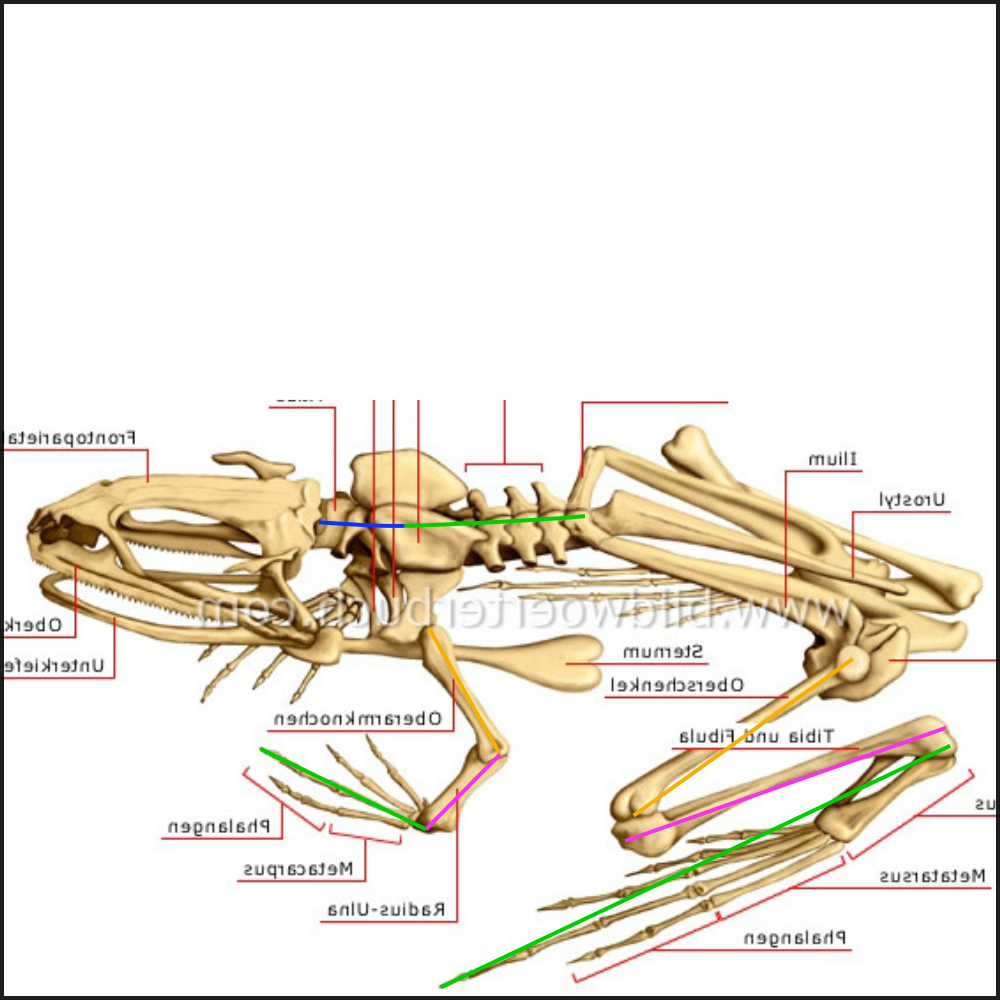
\includegraphics[width=0.5\textwidth]{../PCA/Skelettbilder/Frosch_farbig.png}}
  
  \caption{Frosch (a) Rekonstruktion aus den größten $7$ Eigenvektoren, (b) Eingabebild, zusätzlich erhobene Daten sind:
  Tierklasse: Amphib, keine Flügel, Paare von Beinen mit Bodenkontakt: $2$, ungefähres Gewicht: $0,01$kg}
  \label{frosch}
 \end{figure}
 

 In den Abbildungen, die die Eingabedaten im transformierten Koordinatensystem der PCA darstellen (Abbildung \ref{projections_tags}) ist gut zu erkennen, dass die Koordinatentransformation der PCA die Daten tatsächlich nach den Hauptachsen des mehrdimensionalen Ellipsoids, den die Datenpunkte bilden, ausrichtet.

 Bei allen Eingabedimension, außer der Position der Wirbelsäule, kann man sich die Frage stellen, ob sie nötig sind, oder ob sie eher die Ergebnisse der PCA verschlechtern. Es wurde ausprobiert verschiedene (Kombinationen von) Merkmalen wegzulassen. Die Ergebnisse unterscheiden sich nicht extrem von der PCA mit allen Daten. 
 
 Leider gibt es keine gute Möglichkeit die Qualität der Ergebnisse der PCA zu messen. Man könnte den Unterschied zwischen den Eingabedaten und den Rekonstruktionen aus den Linearkombinationen der Eigenvektoren mit den größten Eigenwerten messen. Aber das liefert, durch das Fehlen von verschiedenen Dimensionen kein einheitliches Maß.
 
 Da jede Dimension dem Algorithmus, der später Skelette generieren soll, helfen könnte, haben wir uns dafür entschieden alle Merkmale zu behalten.
 
 Außerdem gibt es die Möglichkeit die Eingabedaten in mehrere Mengen aufzuteilen und diese von verschiedenen Instanzen der PCA analysieren zu lassen. Hierbei gibt es zunächst das Problem, dass sich dann die Anzahl der Datenpunkte noch weiter reduziert, was die Ergebnisse nicht mehr repräsentativ macht.
 Ein Merkmal, das sich zur Unterteilung in Mengen anbieten würde, ist die Angabe ob das Tier Flügel hat oder nicht, da sich dadurch nur zwei Gruppen ergeben. Außerdem ist die Gruppe der Tiere mit Flügeln in den Eingabedaten bei anderen Skalierungen (siehe Abbildung \ref{projections_scales}) klar als Cluster zu erkennen (siehe auch Abschnitt \ref{pca_input_analysis}). Tatsächlich liefert eine solche Aufteilung bessere Rekonstruktionen aus der größten Eigenvektoren, aber das liegt natürlich vor allem daran, dass die zu untersuchende Datenmenge, jeweils verkleinert wurde.
 
 Ein Problem dabei ist, dass dann keine Skelette mehr erzeugt werden können, die zwischen den beiden Gruppen liegen. Tatsächlich scheinen die Datenpunkte, die "`zwischen"' den Gruppen erzeugt werden, relativ sinnvoll auszusehen.
 Das wäre ein Argument dafür keine Aufteilung vorzunehmen. Dasselbe gilt für die Cluster, die durch die Aufteilung anhand der Anzahl der Beine mit Bodenkontakt entstehen.
 
 \todo{Schaubild mit verschiedenen erzeugten Wirbelsäulen?}
 
 %-------------------------------------------------
 \section{Bedingte Verteilung der PCA Eingabedaten}
 
 
 Aus den Ergebnissen der PCA lassen sich sehr gut zufällige Skelette erzeugen. Es ist aber schwer gezielt Eigenschaften festzulegen.
 Der erste Schritt ist Eigenschaften auf gewählte Werte festzulegen, die so schon in den erhobenen Daten vorkommen. Das können beispielsweise die Anzahl der Beine sein oder ob das Skelett Flügel haben soll.
 
 Dazu kann man, statt die ursprünglichen Daten und deren Verteilung zu verwenden, die bedingten Verteilungen bilden. Dazu muss der bedingte Mittelwert und die bedingte Kovarianzmatrix bestimmt werden.
 
 \todo{Berechnung beschreiben: \url{https://en.wikipedia.org/wiki/Multivariate_normal_distribution#Conditional_distributions}}
 Verwendet man nun die bedingte Kovarianzmatrix als Eingabe für die PCA, so erhält man nur noch Daten für Skelette mit den vorher festgelegten Bedingungen. Zu beachten ist hier, dass die Eigenvektoren sich im Vergleich zur PCA ohne Bedingungen verändern. Falls man diese also zur Bestimmung eines Datenpunktes verwendet hat (\zb in einer Benutzeroberfläche), so müssen die Werte für die neuen Eigenvektoren ganz neu ausgerechnet werden. \todo{ist das relevant für mein Benutzerinterface?}
 
 % feste Werte variieren
 Betrachtet man erzeugte Beispiele aus bedingten Verteilungen, zeigt sich sehr deutlich, dass das Festlegen einer Dimension auch die anderen Dimensionen sehr stark einschränkt. Legt man \zb die Anzahl der Beine fest, so haben die Skelette, die dann bedingt zufällig generiert werden, eine recht geringe Varianz. Das ist deutlich daran zu erkennen, dass der Verlauf der Wirbelsäule immer sehr ähnlich ist.

 Um das etwas zu umgehen, wird die Eingabe als Intervall aufgefasst, aus dem zufällig ein Wert gezogen wird. Legt \zb der Benutzer einen ganzzahligen Wert fest, so wird ein kleiner zufälliger Wert aufaddiert oder abgezogen. \todo{welches Intervall?} So wird nicht immer genau der gleiche Wert verwendet.
 
 % Übergang Krokodil -> Fisch
 Schaut man sich nun die erzeugten Skelette mit zwei tragenden Beinen an, so sind darunter nicht nur Vögel, sondern auch Skelette, die kurze Extremitäten haben und deren Wirbelsäule sich nahe über dem Boden befindet. \todo{Beispielbild}
 Das liegt daran, dass es einen Übergang von bodennahen Vierbeinern wie Krokodilen oder Fröschen zu Fischen geben muss. Da es hier aber in der Natur eher wenige Beispiele für Zweibeiner gibt (in den erhobenen Daten sind das nur der Seehund und die Ohrenrobbe), wirkten diese Tiere eher ungewöhnlich.
 Da das Problem hier aber inhärent in der Vorgehensweise der PCA ist, lässt es sich nicht wirklich beheben.
 
 % Bedingungen an abgeleitet Werte
 Nun möchte man vielleicht Bedingungen an das zu generierende Skelett stellen, die nicht schon genau so in den erhobenen Daten repräsentiert sind. Das könnten beispielsweise die Schwanz- oder Halslänge sein.
 
 Sind es Bedingungen an Dimensionen, die nicht erhoben wurden, können  sie entweder, unabhängig von der PCA, in den Ersetzungsregeln erzwungen werden, wie \zb die Anzahl der Flossen, oder sie müssen in die Erhebung eingefügt werden.
 
 Für Bedingungen, die schon implizit in den erhobenen Daten enthalten sind,
 könnte man es ebenso machen und einfach eine zusätzliche Dimension einfügen, die aus schon bestehenden Dimensionen errechnet wird. Dabei wäre aber das Problem, dass nur die Dimensionalität erhöht wird, nicht aber die eingegebenen Daten. Es wären also mehr Eingabebeispiele nötig, nur dafür, dass die PCA eine offensichtliche Korrelation der Dimensionen erkennt.
 
 Die bessere Alternative ist es die Eingabedimensionen der PCA umzuparametrisieren. Die Länge des Schwanzes in x-Richtung, ist \zb implizit in der Differenz der x-Koordinaten des ersten und letzten Kontrollpunktes der Bezièrkurve des Schwanzes enthalten. Ersetzt man nun den absoluten x-Wert des letzten Kontrollpunktes durch den Abstand in x-Richtung zum ersten Kontrollpunkt, so lässt sich die Schwanzlänge in x-Richtung ganz einfach als Bedingung an die PCA stellen. 
 
 % Schwanzlänge messen
 Betrachtet man nun konkret den Wunsch die Schwanzlänge festzulegen, ist das nicht ganz so einfach. Die Länge in x- und y-Richtung lässt sich zwar leicht festlegen, diese Länge sagen aber noch nicht unbedingt viel über die tatsächliche Länge der Bezièrkurve aus. Verlangt man \zb eine Länge von null für den Schwanz in x-Richtung, so haben die generierten Skelette einen Schwanz der zwar auf gleicher Höhe beginnt und endet, aber trotzdem vorhanden ist und einen kleinen Bogen beschreibt. \todo{Beispielbild}
 Um die wirkliche Länge des Schwanzes zu messen, müsste man also noch mehr Aufwand in die Umparametrisierung stecken oder doch eine zusätzliche Dimension für die PCA in Kauf nehmen.
 
 
